% 174-22(174쪽) — 정삼각형 모양 종이에서 각 변의 중점을 이어 중앙의 정삼각형을 오려낸 1회 시행 뒤의 모습(색칠한 정삼각형 3개).
% 스캔 그림이 흐려 TikZ 로 다시 그렸다. 원문 그림에 없는 값(넓이)은 적지 않는다.
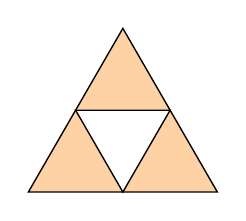
\begin{tikzpicture}[scale=0.8, line width=0.5pt]
  \coordinate (B) at (0,0);
  \coordinate (C) at (3,0);
  \coordinate (A) at (1.5,2.598);
  \coordinate (D) at (0.75,1.299);
  \coordinate (E) at (2.25,1.299);
  \coordinate (F) at (1.5,0);
  \fill[orange!35] (A) -- (D) -- (E) -- cycle;
  \fill[orange!35] (B) -- (F) -- (D) -- cycle;
  \fill[orange!35] (F) -- (C) -- (E) -- cycle;
  \draw (A) -- (B) -- (C) -- cycle;
  \draw (D) -- (E) -- (F) -- cycle;
\end{tikzpicture}
